\onecolumn % go back to one column
\fancyhead{} % make sure we get no headers
\renewcommand{\floatpagefraction}{0.1}
\lfoot[\bSupInf]{\dAuthor}
\rfoot[\dAuthor]{\cSupInf}
\newpage

\captionsetup*{format=largeformat} % make figure legend slightly larger than in the paper
\setcounter{figure}{0} % reset figure counter for Supp. Figures
\setcounter{equation}{0} % reset equation counter for Supp. Equations
\setcounter{table}{0} % reset equation counter for Supp. Equations
\setcounter{page}{1} % reset page count
\makeatletter
\renewcommand{\thefigure}{S\@arabic\c@figure} % make Figure legend start with Figure S
\renewcommand{\thetable}{S\@arabic\c@table} % make Figure legend start with Figure S
\makeatother
\def\theequation{S\arabic{equation}}

\newpage
\section*{Supplementary Information}\label{sec:supplementary-information}

\begin{figure*}[!ht]
	\centering
	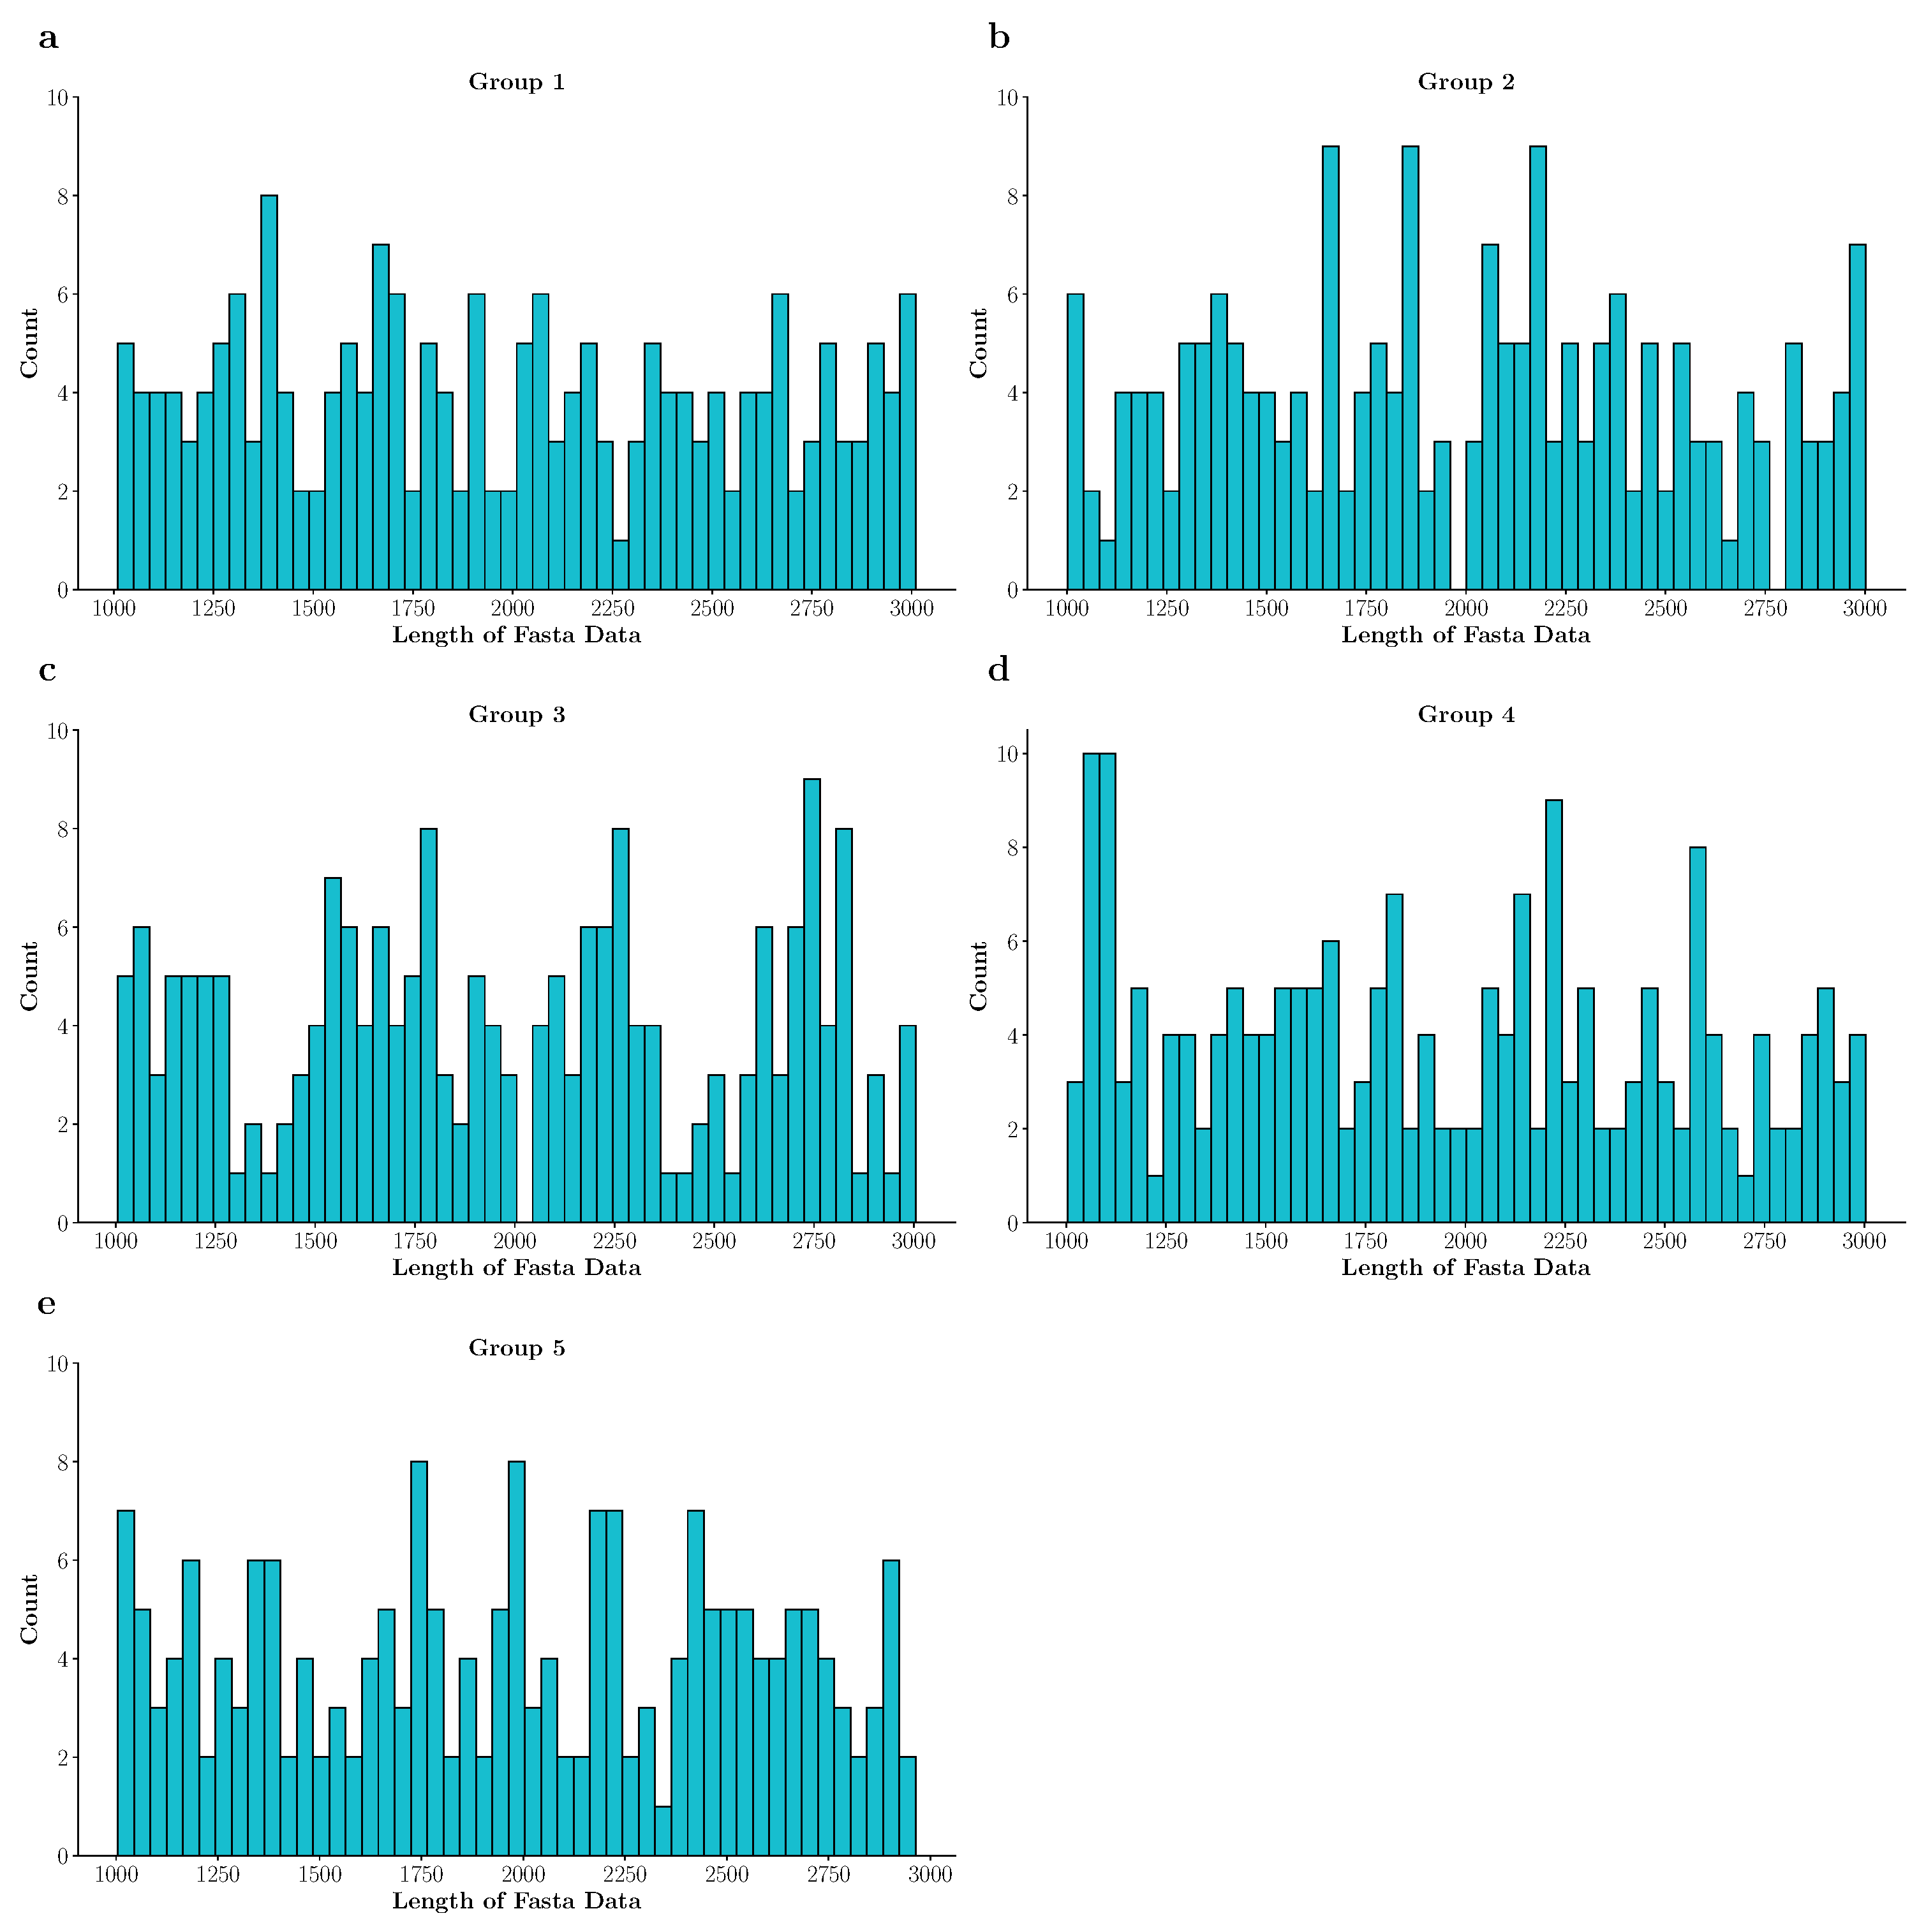
\includegraphics[width=\linewidth]{figures/fas_len.eps}
	\mycaption{Distribution of Sequence Length}{The dataset for testing and benchmarking. Each group contains \num{200} fasta samples, and each fasta sample has one sequence.
		(\textbf{a}) The distribution of length in group \num[round-mode=places, round-precision=0]{1}
		(\textbf{b}) The distribution of length in group \num[round-mode=places, round-precision=0]{2}
		(\textbf{c}) The distribution of length in group \num[round-mode=places, round-precision=0]{3}
		(\textbf{d}) The distribution of length in group \num[round-mode=places, round-precision=0]{4}
		(\textbf{e}) The distribution of length in group \num[round-mode=places, round-precision=0]{5}
	}
	\label{suppfig:fas-len}
\end{figure*}


\begin{longtable}{lSS}
	\caption{Comparison of \glspl{hsp} between BLAT and PxBLAT} \label{supptab:cmp1} \\
	\toprule
	Data                    & {BLAT} & {PxBLAT}                            \\
	\midrule
	\endfirsthead
	\caption[]{Comparison of \glspl{hsp} between BLAT and PxBLAT}                         \\
	\toprule
	Data                    & {BLAT} & {PxBLAT}                            \\
	\midrule
	\endhead
	\midrule
	\multicolumn{3}{r}{Continued on next page}                             \\
	\midrule
	\endfoot
	\bottomrule
	\endlastfoot
	chr20-11648866-11650925 & 130    & 130                                 \\
	chr20-29850079-29852595 & 1      & 1                                   \\
	chr20-7493878-7496145   & 26     & 26                                  \\
	chr20-30152074-30153892 & 3      & 3                                   \\
	chr20-1140095-1141788   & 22     & 22                                  \\
	chr20-17520690-17523557 & 14     & 14                                  \\
	chr20-41374266-41376291 & 12     & 12                                  \\
	chr20-63240773-63243242 & 64     & 64                                  \\
	chr20-59286740-59288091 & 13     & 13                                  \\
	chr20-8061734-8063508   & 10     & 10                                  \\
	chr20-34429296-34431248 & 41     & 41                                  \\
	chr20-27977914-27979241 & 22     & 22                                  \\
	chr20-11695455-11697457 & 20     & 20                                  \\
	chr20-41792348-41794797 & 131    & 131                                 \\
	chr20-25858004-25860351 & 37     & 37                                  \\
	chr20-31404034-31407027 & 25     & 25                                  \\
	chr20-15852904-15855300 & 65     & 65                                  \\
	chr20-29917054-29919227 & 18     & 18                                  \\
	chr20-45175162-45177033 & 2      & 2                                   \\
	chr20-43937342-43939507 & 58     & 58                                  \\
	chr20-17073859-17076499 & 48     & 48                                  \\
	chr20-19823346-19824950 & 32     & 32                                  \\
	chr20-28295597-28298301 & 23     & 23                                  \\
	chr20-15826504-15829187 & 26     & 26                                  \\
	chr20-54683378-54684991 & 47     & 47                                  \\
	chr20-55475241-55476377 & 18     & 18                                  \\
	chr20-57949934-57952283 & 74     & 74                                  \\
	chr20-14442978-14444604 & 35     & 35                                  \\
	chr20-51293808-51295630 & 38     & 38                                  \\
	chr20-49194155-49196823 & 165    & 165                                 \\
	chr20-34696351-34697788 & 43     & 43                                  \\
	chr20-16044321-16045712 & 48     & 48                                  \\
	chr20-45309757-45312553 & 39     & 39                                  \\
	chr20-21063232-21065145 & 26     & 26                                  \\
	chr20-434138-436331     & 174    & 174                                 \\
	chr20-62110486-62112604 & 167    & 167                                 \\
	chr20-15866914-15868171 & 15     & 15                                  \\
	chr20-62343940-62345043 & 69     & 69                                  \\
	chr20-37168356-37170160 & 34     & 34                                  \\
	chr20-15699683-15701260 & 15     & 15                                  \\
	chr20-44826183-44827333 & 152    & 152                                 \\
	chr20-41538435-41540074 & 43     & 43                                  \\
	chr20-56032843-56034378 & 18     & 18                                  \\
	chr20-36813618-36816516 & 21     & 21                                  \\
	chr20-18637848-18640751 & 68     & 68                                  \\
	chr20-56294086-56296598 & 27     & 27                                  \\
	chr20-19514094-19515343 & 2      & 2                                   \\
	chr20-33893321-33895564 & 126    & 126                                 \\
	chr20-22282380-22283429 & 4      & 4                                   \\
	chr20-39910629-39912740 & 84     & 84                                  \\
	chr20-40898874-40901542 & 27     & 27                                  \\
	chr20-7536153-7537696   & 15     & 15                                  \\
	chr20-4818626-4819858   & 60     & 60                                  \\
	chr20-64316707-64319236 & 24     & 24                                  \\
	chr20-2960440-2961833   & 119    & 119                                 \\
	chr20-2519249-2521676   & 46     & 46                                  \\
	chr20-11596878-11599706 & 68     & 68                                  \\
	chr20-30829536-30831739 & 16     & 16                                  \\
	chr20-45188854-45190558 & 3      & 3                                   \\
	chr20-47238745-47241145 & 14     & 14                                  \\
	chr20-10538965-10540232 & 83     & 83                                  \\
	chr20-11996320-11998343 & 87     & 87                                  \\
	chr20-23440919-23442976 & 47     & 47                                  \\
	chr20-22451495-22453568 & 4      & 4                                   \\
	chr20-39709672-39711911 & 23     & 23                                  \\
	chr20-29782708-29784088 & 8      & 8                                   \\
	chr20-7911434-7913178   & 9      & 9                                   \\
	chr20-1508550-1511129   & 193    & 193                                 \\
	chr20-41451172-41452837 & 6      & 6                                   \\
	chr20-4003988-4006545   & 29     & 29                                  \\
	chr20-10921197-10923149 & 5      & 5                                   \\
	chr20-36789016-36790500 & 186    & 186                                 \\
	chr20-9309222-9310479   & 157    & 157                                 \\
	chr20-52532795-52534564 & 9      & 9                                   \\
	chr20-42081563-42082983 & 4      & 4                                   \\
	chr20-12605319-12606971 & 2      & 2                                   \\
	chr20-29389010-29390598 & 149    & 149                                 \\
	chr20-8128132-8130266   & 170    & 170                                 \\
	chr20-11399422-11401237 & 12     & 12                                  \\
	chr20-33251227-33252414 & 2      & 2                                   \\
	chr20-3342256-3343645   & 92     & 92                                  \\
	chr20-38869283-38872088 & 60     & 60                                  \\
	chr20-7649152-7650444   & 60     & 60                                  \\
	chr20-13021673-13023769 & 58     & 58                                  \\
	chr20-3971117-3972667   & 32     & 32                                  \\
	chr20-26232703-26234929 & 61     & 61                                  \\
	chr20-23063517-23064745 & 7      & 7                                   \\
	chr20-39079691-39080763 & 26     & 26                                  \\
	chr20-23882126-23884119 & 92     & 92                                  \\
	chr20-3170215-3172728   & 44     & 44                                  \\
	chr20-49421601-49423499 & 35     & 35                                  \\
	chr20-55380779-55383730 & 204    & 204                                 \\
	chr20-45794728-45796900 & 164    & 164                                 \\
	chr20-15159613-15161221 & 9      & 9                                   \\
	chr20-62378279-62380174 & 184    & 184                                 \\
	chr20-6934771-6936584   & 116    & 116                                 \\
	chr20-59538484-59541329 & 8      & 8                                   \\
	chr20-43661982-43664714 & 26     & 26                                  \\
	chr20-36707842-36709247 & 85     & 85                                  \\
	chr20-33898085-33900435 & 65     & 65                                  \\
	chr20-18062688-18064265 & 46     & 46                                  \\
	chr20-29490152-29491491 & 23     & 23                                  \\
	chr20-11837593-11840377 & 40     & 40                                  \\
	chr20-28934655-28937276 & 1      & 1                                   \\
	chr20-7689471-7691553   & 18     & 18                                  \\
	chr20-1746811-1749803   & 9      & 9                                   \\
	chr20-1261408-1262588   & 16     & 16                                  \\
	chr20-5757029-5759548   & 29     & 29                                  \\
	chr20-5361957-5364278   & 107    & 107                                 \\
	chr20-37305589-37308001 & 21     & 21                                  \\
	chr20-53702835-53705300 & 148    & 148                                 \\
	chr20-7447290-7449191   & 16     & 16                                  \\
	chr20-36626015-36629010 & 150    & 150                                 \\
	chr20-48184357-48185678 & 2      & 2                                   \\
	chr20-4634043-4636057   & 9      & 9                                   \\
	chr20-21292878-21295830 & 179    & 179                                 \\
	chr20-52551672-52553086 & 7      & 7                                   \\
	chr20-55410142-55411547 & 55     & 55                                  \\
	chr20-15164296-15166007 & 21     & 21                                  \\
	chr20-60294852-60297789 & 197    & 197                                 \\
	chr20-47112993-47114241 & 38     & 38                                  \\
	chr20-33645643-33648541 & 62     & 62                                  \\
	chr20-57099663-57101555 & 91     & 91                                  \\
	chr20-32443012-32444528 & 1      & 1                                   \\
	chr20-54597242-54598325 & 31     & 31                                  \\
	chr20-28168758-28171348 & 20     & 20                                  \\
	chr20-14255274-14256294 & 211    & 211                                 \\
	chr20-22858139-22859797 & 8      & 8                                   \\
	chr20-42977157-42978222 & 11     & 11                                  \\
	chr20-3890553-3891667   & 46     & 46                                  \\
	chr20-10043505-10044872 & 33     & 33                                  \\
	chr20-47292153-47293840 & 50     & 50                                  \\
	chr20-23406092-23408775 & 15     & 15                                  \\
	chr20-44245002-44246392 & 36     & 36                                  \\
	chr20-30999482-31002350 & 1      & 1                                   \\
	chr20-11990150-11991239 & 3      & 3                                   \\
	chr20-3810992-3812466   & 197    & 197                                 \\
	chr20-22091287-22094021 & 119    & 119                                 \\
	chr20-47477509-47479589 & 59     & 59                                  \\
	chr20-13750647-13753070 & 44     & 44                                  \\
	chr20-61483678-61484972 & 2      & 2                                   \\
	chr20-57584630-57586794 & 13     & 13                                  \\
	chr20-17904728-17906925 & 34     & 34                                  \\
	chr20-28086098-28087474 & 19     & 19                                  \\
	chr20-21317295-21318548 & 51     & 51                                  \\
	chr20-42758324-42759488 & 193    & 193                                 \\
	chr20-23580801-23581810 & 23     & 23                                  \\
	chr20-58929386-58930631 & 22     & 22                                  \\
	chr20-6605062-6607136   & 79     & 79                                  \\
	chr20-32987534-32989963 & 169    & 169                                 \\
	chr20-22493043-22494805 & 22     & 22                                  \\
	chr20-54190709-54192035 & 24     & 24                                  \\
	chr20-48343887-48346044 & 2      & 2                                   \\
	chr20-10262876-10265171 & 189    & 189                                 \\
	chr20-35374558-35376267 & 67     & 67                                  \\
	chr20-39018648-39021540 & 83     & 83                                  \\
	chr20-37785924-37788264 & 202    & 202                                 \\
	chr20-12575681-12578297 & 14     & 14                                  \\
	chr20-23374273-23375283 & 1      & 1                                   \\
	chr20-14278920-14280350 & 40     & 40                                  \\
	chr20-42778102-42780755 & 9      & 9                                   \\
	chr20-52810557-52811573 & 83     & 83                                  \\
	chr20-52564945-52566606 & 22     & 22                                  \\
	chr20-10598821-10601808 & 32     & 32                                  \\
	chr20-1172826-1175431   & 87     & 87                                  \\
	chr20-3347653-3350627   & 44     & 44                                  \\
	chr20-64176870-64179763 & 43     & 43                                  \\
	chr20-42829128-42830258 & 100    & 100                                 \\
	chr20-40623645-40625957 & 187    & 187                                 \\
	chr20-27009229-27011878 & 24     & 24                                  \\
	chr20-14732847-14734481 & 95     & 95                                  \\
	chr20-12698635-12699679 & 2      & 2                                   \\
	chr20-13328590-13330614 & 13     & 13                                  \\
	chr20-22912395-22915205 & 12     & 12                                  \\
	chr20-35339375-35342113 & 48     & 48                                  \\
	chr20-19431509-19433187 & 28     & 28                                  \\
	chr20-28727730-28729750 & 16     & 16                                  \\
	chr20-39515806-39517118 & 2      & 2                                   \\
	chr20-21857448-21859310 & 209    & 209                                 \\
	chr20-44751640-44753567 & 19     & 19                                  \\
	chr20-47371415-47374127 & 45     & 45                                  \\
	chr20-24140371-24142959 & 6      & 6                                   \\
	chr20-54083025-54084528 & 41     & 41                                  \\
	chr20-51775800-51777458 & 46     & 46                                  \\
	chr20-59400225-59402632 & 30     & 30                                  \\
	chr20-57144627-57147621 & 47     & 47                                  \\
	chr20-17690928-17692128 & 6      & 6                                   \\
	chr20-31238605-31240139 & 4      & 4                                   \\
	chr20-29259215-29262074 & 4      & 4                                   \\
	chr20-39132690-39134466 & 34     & 34                                  \\
	chr20-44674003-44676622 & 31     & 31                                  \\
	chr20-34435089-34436815 & 13     & 13                                  \\
	chr20-11085268-11087065 & 27     & 27                                  \\
	chr20-42010931-42012642 & 10     & 10                                  \\
	chr20-7483012-7484115   & 1      & 1                                   \\
	chr20-39873233-39875635 & 207    & 207                                 \\
\end{longtable}


\begin{longtable}{lSS}
	\caption{Comparison between BLAT and PxBLAT} \label{tab:cmp2} \\
	\toprule
	Data                    & {BLAT} & {PxBLAT}                   \\
	\midrule
	\endfirsthead
	\caption[]{Comparison between BLAT and PxBLAT}                \\
	\toprule
	Data                    & {BLAT} & {PxBLAT}                   \\
	\midrule
	\endhead
	\midrule
	\multicolumn{3}{r}{Continued on next page}                    \\
	\midrule
	\endfoot
	\bottomrule
	\endlastfoot
	chr20-2828159-2830288   & 134    & 134                        \\
	chr20-8971949-8973716   & 18     & 18                         \\
	chr20-30095884-30097442 & 17     & 17                         \\
	chr20-51719657-51722053 & 173    & 173                        \\
	chr20-33974288-33975838 & 69     & 69                         \\
	chr20-2278332-2280708   & 15     & 15                         \\
	chr20-3395428-3397753   & 86     & 86                         \\
	chr20-63803154-63805985 & 43     & 43                         \\
	chr20-48031931-48034204 & 44     & 44                         \\
	chr20-46308727-46309965 & 6      & 6                          \\
	chr20-14083167-14084282 & 167    & 167                        \\
	chr20-45353941-45356038 & 53     & 53                         \\
	chr20-63851619-63854055 & 64     & 64                         \\
	chr20-50583738-50585129 & 3      & 3                          \\
	chr20-13751249-13752454 & 42     & 42                         \\
	chr20-49452302-49454684 & 159    & 159                        \\
	chr20-18383256-18384901 & 73     & 73                         \\
	chr20-29651400-29652794 & 9      & 9                          \\
	chr20-40330327-40331786 & 18     & 18                         \\
	chr20-35818754-35821105 & 100    & 100                        \\
	chr20-2688118-2690258   & 39     & 39                         \\
	chr20-47399940-47402884 & 114    & 114                        \\
	chr20-50899780-50901977 & 19     & 19                         \\
	chr20-43133225-43135909 & 192    & 192                        \\
	chr20-46544773-46547501 & 10     & 10                         \\
	chr20-19754747-19756349 & 18     & 18                         \\
	chr20-223022-225549     & 9      & 9                          \\
	chr20-63046239-63049189 & 47     & 47                         \\
	chr20-57304541-57306258 & 58     & 58                         \\
	chr20-38493743-38495091 & 25     & 25                         \\
	chr20-20265635-20267968 & 16     & 16                         \\
	chr20-2844781-2847151   & 93     & 93                         \\
	chr20-53725027-53727516 & 36     & 36                         \\
	chr20-10920657-10922515 & 8      & 8                          \\
	chr20-44371315-44374295 & 39     & 39                         \\
	chr20-3431376-3433251   & 202    & 202                        \\
	chr20-39135488-39137700 & 52     & 52                         \\
	chr20-58745286-58747067 & 11     & 11                         \\
	chr20-31791374-31793816 & 205    & 205                        \\
	chr20-36971580-36972630 & 27     & 27                         \\
	chr20-45741446-45744259 & 26     & 26                         \\
	chr20-28837189-28840052 & 1      & 1                          \\
	chr20-53642354-53643485 & 103    & 103                        \\
	chr20-63846146-63848461 & 16     & 16                         \\
	chr20-24600426-24602535 & 54     & 54                         \\
	chr20-12493566-12496209 & 178    & 178                        \\
	chr20-24425863-24428862 & 24     & 24                         \\
	chr20-43710550-43713461 & 126    & 126                        \\
	chr20-3694835-3697763   & 73     & 73                         \\
	chr20-49087699-49089567 & 8      & 8                          \\
	chr20-51447199-51448636 & 88     & 88                         \\
	chr20-8640913-8642978   & 6      & 6                          \\
	chr20-53874690-53877592 & 56     & 56                         \\
	chr20-32558083-32560533 & 37     & 37                         \\
	chr20-39866491-39868448 & 32     & 32                         \\
	chr20-57235806-57237280 & 2      & 2                          \\
	chr20-1551870-1553269   & 2      & 2                          \\
	chr20-60276391-60278170 & 31     & 31                         \\
	chr20-47735701-47737760 & 12     & 12                         \\
	chr20-47950200-47952033 & 26     & 26                         \\
	chr20-37264292-37266206 & 95     & 95                         \\
	chr20-25972909-25975750 & 5      & 5                          \\
	chr20-49810048-49811680 & 22     & 22                         \\
	chr20-7730740-7733285   & 45     & 45                         \\
	chr20-51212931-51215436 & 46     & 46                         \\
	chr20-35679220-35680810 & 178    & 178                        \\
	chr20-60278816-60280383 & 4      & 4                          \\
	chr20-1848711-1850476   & 89     & 89                         \\
	chr20-61487368-61489909 & 64     & 64                         \\
	chr20-37154283-37155740 & 35     & 35                         \\
	chr20-10295968-10296987 & 7      & 7                          \\
	chr20-61931058-61933207 & 7      & 7                          \\
	chr20-59480418-59482175 & 191    & 191                        \\
	chr20-47105521-47106711 & 109    & 109                        \\
	chr20-28467685-28469748 & 20     & 20                         \\
	chr20-23363427-23366158 & 26     & 26                         \\
	chr20-1681181-1682213   & 28     & 28                         \\
	chr20-23846256-23847406 & 31     & 31                         \\
	chr20-55274707-55276347 & 223    & 223                        \\
	chr20-63347021-63349649 & 4      & 4                          \\
	chr20-40080433-40082317 & 75     & 75                         \\
	chr20-9530092-9532401   & 1      & 1                          \\
	chr20-38108034-38110387 & 56     & 56                         \\
	chr20-9623861-9625540   & 5      & 5                          \\
	chr20-58197693-58200651 & 48     & 48                         \\
	chr20-14255898-14258880 & 13     & 13                         \\
	chr20-29162172-29164046 & 18     & 18                         \\
	chr20-3651661-3653661   & 19     & 19                         \\
	chr20-54221532-54223373 & 24     & 24                         \\
	chr20-30550507-30552616 & 3      & 3                          \\
	chr20-54778098-54779435 & 3      & 3                          \\
	chr20-34554504-34557124 & 195    & 195                        \\
	chr20-46153137-46156011 & 61     & 61                         \\
	chr20-19287160-19289355 & 61     & 61                         \\
	chr20-15370716-15372514 & 6      & 6                          \\
	chr20-12817209-12820043 & 213    & 213                        \\
	chr20-26494131-26495614 & 26     & 26                         \\
	chr20-44385075-44387095 & 34     & 34                         \\
	chr20-30229549-30231195 & 216    & 216                        \\
	chr20-58407287-58410250 & 54     & 54                         \\
	chr20-22419707-22421972 & 5      & 5                          \\
	chr20-64189992-64192899 & 44     & 44                         \\
	chr20-60602761-60605519 & 57     & 57                         \\
	chr20-29075089-29077901 & 22     & 22                         \\
	chr20-51434881-51436198 & 39     & 39                         \\
	chr20-29854637-29855989 & 3      & 3                          \\
	chr20-29127537-29128926 & 16     & 16                         \\
	chr20-3190191-3192877   & 35     & 35                         \\
	chr20-35916578-35918313 & 59     & 59                         \\
	chr20-56918427-56920492 & 34     & 34                         \\
	chr20-41848804-41850751 & 2      & 2                          \\
	chr20-26793231-26795382 & 22     & 22                         \\
	chr20-64014289-64015618 & 42     & 42                         \\
	chr20-39382394-39384063 & 6      & 6                          \\
	chr20-11297686-11298759 & 29     & 29                         \\
	chr20-53600600-53601859 & 25     & 25                         \\
	chr20-7664191-7666587   & 117    & 117                        \\
	chr20-50657586-50658971 & 43     & 43                         \\
	chr20-14086263-14087689 & 27     & 27                         \\
	chr20-31644053-31645876 & 202    & 202                        \\
	chr20-49881247-49883414 & 19     & 19                         \\
	chr20-39045849-39048318 & 71     & 71                         \\
	chr20-26667702-26668733 & 24     & 24                         \\
	chr20-35794840-35797816 & 33     & 33                         \\
	chr20-14041285-14043655 & 43     & 43                         \\
	chr20-43887719-43889010 & 77     & 77                         \\
	chr20-48557745-48559863 & 75     & 75                         \\
	chr20-13636473-13637790 & 22     & 22                         \\
	chr20-60386487-60388629 & 85     & 85                         \\
	chr20-46602679-46604724 & 105    & 105                        \\
	chr20-6342124-6344048   & 2      & 2                          \\
	chr20-52509804-52511365 & 24     & 24                         \\
	chr20-8596729-8597957   & 184    & 184                        \\
	chr20-46229584-46231629 & 10     & 10                         \\
	chr20-32426330-32428027 & 49     & 49                         \\
	chr20-59309503-59310835 & 26     & 26                         \\
	chr20-44725323-44726823 & 169    & 169                        \\
	chr20-3932045-3934068   & 4      & 4                          \\
	chr20-923271-925546     & 23     & 23                         \\
	chr20-8844646-8845932   & 118    & 118                        \\
	chr20-16341258-16343778 & 11     & 11                         \\
	chr20-11253087-11254915 & 6      & 6                          \\
	chr20-62299195-62300925 & 16     & 16                         \\
	chr20-13574193-13576883 & 36     & 36                         \\
	chr20-47318361-47320801 & 67     & 67                         \\
	chr20-38097496-38099695 & 110    & 110                        \\
	chr20-16852028-16854617 & 9      & 9                          \\
	chr20-48876739-48878931 & 38     & 38                         \\
	chr20-46598465-46599826 & 9      & 9                          \\
	chr20-50733724-50735913 & 31     & 31                         \\
	chr20-16694673-16696959 & 41     & 41                         \\
	chr20-60554396-60556059 & 3      & 3                          \\
	chr20-7100666-7102477   & 22     & 22                         \\
	chr20-9052261-9055087   & 202    & 202                        \\
	chr20-47716012-47718585 & 49     & 49                         \\
	chr20-55091558-55093023 & 18     & 18                         \\
	chr20-55647967-55649485 & 37     & 37                         \\
	chr20-12070860-12072133 & 201    & 201                        \\
	chr20-46040466-46042741 & 17     & 17                         \\
	chr20-59258885-59260725 & 58     & 58                         \\
	chr20-41615264-41617426 & 6      & 6                          \\
	chr20-47812008-47813426 & 32     & 32                         \\
	chr20-53173457-53174462 & 31     & 31                         \\
	chr20-47785182-47786828 & 10     & 10                         \\
	chr20-17404964-17407937 & 2      & 2                          \\
	chr20-33100162-33102029 & 19     & 19                         \\
	chr20-38669941-38671179 & 89     & 89                         \\
	chr20-24203548-24204576 & 1      & 1                          \\
	chr20-56658618-56660794 & 26     & 26                         \\
	chr20-9502811-9505031   & 39     & 39                         \\
	chr20-444175-446235     & 55     & 55                         \\
	chr20-64042363-64044772 & 66     & 66                         \\
	chr20-42146908-42148554 & 5      & 5                          \\
	chr20-31814615-31816841 & 14     & 14                         \\
	chr20-7185589-7186727   & 23     & 23                         \\
	chr20-4210142-4212478   & 108    & 108                        \\
	chr20-2738418-2740895   & 40     & 40                         \\
	chr20-24397070-24398500 & 172    & 172                        \\
	chr20-62308298-62309851 & 1      & 1                          \\
	chr20-25326590-25328009 & 35     & 35                         \\
	chr20-16727307-16729492 & 45     & 45                         \\
	chr20-38178690-38181407 & 26     & 26                         \\
	chr20-23745409-23746596 & 4      & 4                          \\
	chr20-28209126-28211757 & 22     & 22                         \\
	chr20-14538504-14540773 & 3      & 3                          \\
	chr20-18389195-18390366 & 1      & 1                          \\
	chr20-48698281-48699926 & 90     & 90                         \\
	chr20-17745800-17748778 & 21     & 21                         \\
	chr20-17202460-17203460 & 18     & 18                         \\
	chr20-3858012-3859518   & 62     & 62                         \\
	chr20-38806155-38807719 & 5      & 5                          \\
	chr20-59941646-59943512 & 10     & 10                         \\
	chr20-18936575-18939153 & 12     & 12                         \\
	chr20-45510964-45512824 & 41     & 41                         \\
	chr20-26624053-26625245 & 21     & 21                         \\
	chr20-37191072-37192377 & 38     & 38                         \\
\end{longtable}

\begin{longtable}{lSS}
	\caption{Comparison between BLAT and PxBLAT} \label{tab:cmp3} \\
	\toprule
	Data                    & {BLAT} & {PxBLAT}                   \\
	\midrule
	\endfirsthead
	\caption[]{Comparison between BLAT and PxBLAT}                \\
	\toprule
	Data                    & {BLAT} & {PxBLAT}                   \\
	\midrule
	\endhead
	\midrule
	\multicolumn{3}{r}{Continued on next page}                    \\
	\midrule
	\endfoot
	\bottomrule
	\endlastfoot
	chr20-32029134-32032031 & 93     & 93                         \\
	chr20-38052616-38054138 & 32     & 32                         \\
	chr20-2602976-2605324   & 19     & 19                         \\
	chr20-42169915-42172757 & 15     & 15                         \\
	chr20-62125729-62128471 & 19     & 19                         \\
	chr20-2162753-2164165   & 5      & 5                          \\
	chr20-34630972-34632436 & 113    & 113                        \\
	chr20-6611620-6614440   & 152    & 152                        \\
	chr20-19300360-19302642 & 6      & 6                          \\
	chr20-25189802-25191365 & 154    & 154                        \\
	chr20-15951964-15953450 & 26     & 26                         \\
	chr20-47285001-47287102 & 52     & 52                         \\
	chr20-22548369-22549974 & 9      & 9                          \\
	chr20-24725480-24727693 & 52     & 52                         \\
	chr20-55633941-55636718 & 5      & 5                          \\
	chr20-30324027-30326285 & 30     & 30                         \\
	chr20-34789703-34791591 & 27     & 27                         \\
	chr20-22886111-22887126 & 5      & 5                          \\
	chr20-52373722-52374925 & 52     & 52                         \\
	chr20-62594615-62596270 & 61     & 61                         \\
	chr20-23567798-23569994 & 5      & 5                          \\
	chr20-52746782-52748970 & 26     & 26                         \\
	chr20-63919107-63920159 & 20     & 20                         \\
	chr20-37603411-37606081 & 21     & 21                         \\
	chr20-45549091-45551404 & 167    & 167                        \\
	chr20-24122821-24124880 & 2      & 2                          \\
	chr20-39384970-39386746 & 47     & 47                         \\
	chr20-56953750-56954962 & 11     & 11                         \\
	chr20-27265832-27268665 & 27     & 27                         \\
	chr20-989008-991475     & 96     & 96                         \\
	chr20-13233506-13234845 & 9      & 9                          \\
	chr20-54079315-54081921 & 56     & 56                         \\
	chr20-22276591-22279281 & 202    & 202                        \\
	chr20-32344273-32347087 & 26     & 26                         \\
	chr20-14761627-14763228 & 15     & 15                         \\
	chr20-24471803-24474607 & 7      & 7                          \\
	chr20-22305788-22308754 & 43     & 43                         \\
	chr20-63927315-63929626 & 54     & 54                         \\
	chr20-33534721-33537439 & 158    & 158                        \\
	chr20-53020990-53022920 & 33     & 33                         \\
	chr20-44701412-44703325 & 34     & 34                         \\
	chr20-63523339-63524524 & 190    & 190                        \\
	chr20-39750571-39752199 & 50     & 50                         \\
	chr20-47879542-47880820 & 162    & 162                        \\
	chr20-12949055-12950079 & 1      & 1                          \\
	chr20-37737796-37740734 & 26     & 26                         \\
	chr20-17600492-17603407 & 68     & 68                         \\
	chr20-40848143-40849212 & 2      & 2                          \\
	chr20-33135173-33136880 & 131    & 131                        \\
	chr20-39118192-39119260 & 4      & 4                          \\
	chr20-27690465-27692366 & 23     & 23                         \\
	chr20-37858061-37860321 & 49     & 49                         \\
	chr20-12405605-12407882 & 6      & 6                          \\
	chr20-57386121-57387852 & 70     & 70                         \\
	chr20-34902889-34905611 & 39     & 39                         \\
	chr20-52070637-52073331 & 35     & 35                         \\
	chr20-40779660-40781751 & 47     & 47                         \\
	chr20-31098450-31100717 & 3      & 3                          \\
	chr20-29969458-29971235 & 18     & 18                         \\
	chr20-13789470-13791842 & 152    & 152                        \\
	chr20-26814485-26817257 & 22     & 22                         \\
	chr20-40740691-40742983 & 29     & 29                         \\
	chr20-49955693-49958425 & 183    & 183                        \\
	chr20-37813305-37814584 & 9      & 9                          \\
	chr20-18255943-18258048 & 64     & 64                         \\
	chr20-63109432-63111043 & 34     & 34                         \\
	chr20-14211039-14213272 & 9      & 9                          \\
	chr20-17100441-17103140 & 9      & 9                          \\
	chr20-2866996-2869328   & 38     & 38                         \\
	chr20-53703835-53705398 & 158    & 158                        \\
	chr20-51431118-51433743 & 56     & 56                         \\
	chr20-6192786-6193790   & 196    & 196                        \\
	chr20-10748356-10751019 & 35     & 35                         \\
	chr20-33974548-33976407 & 44     & 44                         \\
	chr20-32270385-32273111 & 20     & 20                         \\
	chr20-36902282-36904506 & 28     & 28                         \\
	chr20-198832-201190     & 40     & 40                         \\
	chr20-7927314-7928574   & 27     & 27                         \\
	chr20-17899461-17900502 & 58     & 58                         \\
	chr20-11120841-11122366 & 23     & 23                         \\
	chr20-59407661-59409193 & 27     & 27                         \\
	chr20-35649824-35652625 & 5      & 5                          \\
	chr20-30688628-30690580 & 48     & 48                         \\
	chr20-49466264-49467309 & 5      & 5                          \\
	chr20-63692672-63694078 & 2      & 2                          \\
	chr20-12570747-12573421 & 5      & 5                          \\
	chr20-8512304-8514491   & 20     & 20                         \\
	chr20-24204303-24205314 & 2      & 2                          \\
	chr20-11639430-11641175 & 20     & 20                         \\
	chr20-26938330-26940788 & 24     & 24                         \\
	chr20-17587799-17589501 & 209    & 209                        \\
	chr20-26384682-26386149 & 23     & 23                         \\
	chr20-46308421-46310414 & 41     & 41                         \\
	chr20-44079162-44081096 & 23     & 23                         \\
	chr20-21475551-21476686 & 50     & 50                         \\
	chr20-13972488-13974627 & 44     & 44                         \\
	chr20-45697903-45699479 & 88     & 88                         \\
	chr20-24838480-24839925 & 11     & 11                         \\
	chr20-7742386-7745111   & 4      & 4                          \\
	chr20-56522851-56524815 & 12     & 12                         \\
	chr20-22497057-22499773 & 16     & 16                         \\
	chr20-51998729-52000293 & 22     & 22                         \\
	chr20-38767581-38768689 & 5      & 5                          \\
	chr20-19863311-19865822 & 56     & 56                         \\
	chr20-9295230-9297764   & 226    & 226                        \\
	chr20-15012779-15015584 & 8      & 8                          \\
	chr20-5041846-5044587   & 56     & 56                         \\
	chr20-580210-582022     & 35     & 35                         \\
	chr20-15328579-15331324 & 42     & 42                         \\
	chr20-49481967-49483214 & 17     & 17                         \\
	chr20-5260817-5262044   & 5      & 5                          \\
	chr20-23340929-23343084 & 102    & 102                        \\
	chr20-2269716-2270774   & 189    & 189                        \\
	chr20-46399947-46401667 & 31     & 31                         \\
	chr20-10815100-10817410 & 32     & 32                         \\
	chr20-45864818-45866440 & 53     & 53                         \\
	chr20-45489949-45492069 & 35     & 35                         \\
	chr20-21302718-21304312 & 1      & 1                          \\
	chr20-9931834-9933992   & 5      & 5                          \\
	chr20-56295194-56296721 & 5      & 5                          \\
	chr20-38225781-38227971 & 18     & 18                         \\
	chr20-18585659-18587381 & 35     & 35                         \\
	chr20-16940912-16942721 & 39     & 39                         \\
	chr20-3758200-3759977   & 4      & 4                          \\
	chr20-11807056-11808124 & 3      & 3                          \\
	chr20-127575-129488     & 93     & 93                         \\
	chr20-40755444-40756701 & 5      & 5                          \\
	chr20-21011682-21013735 & 2      & 2                          \\
	chr20-10119043-10120171 & 59     & 59                         \\
	chr20-1313128-1315640   & 18     & 18                         \\
	chr20-11712977-11715178 & 142    & 142                        \\
	chr20-34597997-34600726 & 28     & 28                         \\
	chr20-53048517-53050101 & 29     & 29                         \\
	chr20-15161566-15163488 & 8      & 8                          \\
	chr20-15137364-15139959 & 203    & 203                        \\
	chr20-60342420-60345056 & 94     & 94                         \\
	chr20-55169861-55170982 & 156    & 156                        \\
	chr20-24314101-24316265 & 27     & 27                         \\
	chr20-53183314-53186148 & 16     & 16                         \\
	chr20-43887385-43889661 & 75     & 75                         \\
	chr20-59470391-59471545 & 1      & 1                          \\
	chr20-53159093-53161302 & 35     & 35                         \\
	chr20-5895129-5896312   & 26     & 26                         \\
	chr20-25292499-25293803 & 3      & 3                          \\
	chr20-34161145-34162369 & 41     & 41                         \\
	chr20-45868564-45870103 & 74     & 74                         \\
	chr20-4887453-4889888   & 3      & 3                          \\
	chr20-39559840-39561722 & 9      & 9                          \\
	chr20-33221436-33223116 & 56     & 56                         \\
	chr20-755464-758088     & 35     & 35                         \\
	chr20-1111176-1112831   & 46     & 46                         \\
	chr20-2802607-2803838   & 36     & 36                         \\
	chr20-38997152-38999498 & 22     & 22                         \\
	chr20-5049946-5052675   & 35     & 35                         \\
	chr20-48767423-48769196 & 48     & 48                         \\
	chr20-2659893-2661452   & 56     & 56                         \\
	chr20-49121260-49124086 & 21     & 21                         \\
	chr20-54247731-54250009 & 75     & 75                         \\
	chr20-8334685-8337480   & 34     & 34                         \\
	chr20-1762478-1764560   & 46     & 46                         \\
	chr20-53286968-53289954 & 23     & 23                         \\
	chr20-23613637-23615158 & 53     & 53                         \\
	chr20-7135001-7136753   & 88     & 88                         \\
	chr20-59872605-59875175 & 5      & 5                          \\
	chr20-33944307-33946354 & 27     & 27                         \\
	chr20-29344297-29347205 & 8      & 8                          \\
	chr20-28334593-28336360 & 22     & 22                         \\
	chr20-49230825-49232042 & 66     & 66                         \\
	chr20-48044237-48045631 & 3      & 3                          \\
	chr20-26227485-26229228 & 5      & 5                          \\
	chr20-26487906-26489572 & 25     & 25                         \\
	chr20-11596974-11599728 & 65     & 65                         \\
	chr20-45661385-45663135 & 194    & 194                        \\
	chr20-23562380-23564047 & 2      & 2                          \\
	chr20-5735736-5738602   & 12     & 12                         \\
	chr20-55535504-55537712 & 3      & 3                          \\
	chr20-45493939-45496533 & 99     & 99                         \\
	chr20-25430083-25432571 & 107    & 107                        \\
	chr20-2981029-2982513   & 77     & 77                         \\
	chr20-49523722-49525938 & 32     & 32                         \\
	chr20-27912294-27914399 & 20     & 20                         \\
	chr20-15366252-15368022 & 33     & 33                         \\
	chr20-40846798-40849784 & 29     & 29                         \\
	chr20-20650550-20653192 & 59     & 59                         \\
	chr20-13545370-13547154 & 2      & 2                          \\
	chr20-27596727-27598551 & 19     & 19                         \\
	chr20-3394620-3396590   & 171    & 171                        \\
	chr20-1444330-1446279   & 3      & 3                          \\
	chr20-42147101-42148224 & 2      & 2                          \\
	chr20-60359901-60361245 & 11     & 11                         \\
	chr20-58137613-58139410 & 3      & 3                          \\
	chr20-40224761-40225920 & 10     & 10                         \\
	chr20-57324246-57325405 & 13     & 13                         \\
	chr20-21713213-21715491 & 39     & 39                         \\
	chr20-14037568-14040191 & 83     & 83                         \\
	chr20-16385063-16388039 & 118    & 118                        \\
	chr20-59768230-59769419 & 5      & 5                          \\
\end{longtable}

\begin{longtable}{lSS}
	\caption{Comparison of \glspl{hsp} between BLAT and PxBLAT} \label{supptab:cmp4} \\
	\toprule
	Data                    & {BLAT} & {PxBLAT}                                  \\
	\midrule
	\endfirsthead
	\caption[]{Comparison of \glspl{hsp} between BLAT and PxBLAT}                \\
	\toprule
	Data                    & {BLAT} & {PxBLAT}                                  \\
	\midrule
	\endhead
	\midrule
	\multicolumn{3}{r}{Continued on next page}                                   \\
	\midrule
	\endfoot
	\bottomrule
	\endlastfoot
	chr20-31727237-31729024 & 39     & 39                                        \\
	chr20-36152090-36154966 & 151    & 151                                       \\
	chr20-1018906-1020553   & 11     & 11                                        \\
	chr20-9821106-9823172   & 75     & 75                                        \\
	chr20-52034533-52037144 & 85     & 85                                        \\
	chr20-15008181-15010280 & 66     & 66                                        \\
	chr20-41851737-41853531 & 6      & 6                                         \\
	chr20-29408974-29411107 & 20     & 20                                        \\
	chr20-10955881-10957008 & 1      & 1                                         \\
	chr20-8970270-8971572   & 18     & 18                                        \\
	chr20-2350436-2352589   & 200    & 200                                       \\
	chr20-35494115-35496325 & 37     & 37                                        \\
	chr20-16994461-16996880 & 203    & 203                                       \\
	chr20-1121638-1123536   & 20     & 20                                        \\
	chr20-10539946-10542788 & 76     & 76                                        \\
	chr20-31981394-31984035 & 24     & 24                                        \\
	chr20-31059406-31062015 & 9      & 9                                         \\
	chr20-23005241-23006490 & 85     & 85                                        \\
	chr20-27678668-27680740 & 22     & 22                                        \\
	chr20-23089029-23090440 & 1      & 1                                         \\
	chr20-18766639-18768846 & 74     & 74                                        \\
	chr20-35270491-35271927 & 24     & 24                                        \\
	chr20-32671767-32673927 & 46     & 46                                        \\
	chr20-5469364-5470405   & 1      & 1                                         \\
	chr20-44586665-44588074 & 3      & 3                                         \\
	chr20-19751371-19752469 & 50     & 50                                        \\
	chr20-11475039-11477338 & 4      & 4                                         \\
	chr20-52930875-52933353 & 52     & 52                                        \\
	chr20-23941121-23942933 & 189    & 189                                       \\
	chr20-10612667-10615654 & 16     & 16                                        \\
	chr20-39220431-39222072 & 6      & 6                                         \\
	chr20-24056618-24059198 & 190    & 190                                       \\
	chr20-63753892-63756615 & 196    & 196                                       \\
	chr20-64298054-64301011 & 16     & 16                                        \\
	chr20-43632072-43634462 & 46     & 46                                        \\
	chr20-29402266-29403661 & 49     & 49                                        \\
	chr20-34611441-34612505 & 39     & 39                                        \\
	chr20-16219627-16222599 & 19     & 19                                        \\
	chr20-47623287-47624373 & 18     & 18                                        \\
	chr20-37572653-37574987 & 20     & 20                                        \\
	chr20-57328038-57329145 & 159    & 159                                       \\
	chr20-54255861-54257299 & 11     & 11                                        \\
	chr20-17523656-17525455 & 3      & 3                                         \\
	chr20-3054439-3055812   & 26     & 26                                        \\
	chr20-51095602-51096740 & 8      & 8                                         \\
	chr20-26295259-26296843 & 6      & 6                                         \\
	chr20-16956946-16959866 & 4      & 4                                         \\
	chr20-59871467-59873730 & 18     & 18                                        \\
	chr20-12972124-12973571 & 9      & 9                                         \\
	chr20-64187505-64190371 & 7      & 7                                         \\
	chr20-20036801-20038441 & 54     & 54                                        \\
	chr20-52361579-52363650 & 49     & 49                                        \\
	chr20-48763637-48765211 & 21     & 21                                        \\
	chr20-29272745-29274078 & 3      & 3                                         \\
	chr20-6596603-6597647   & 1      & 1                                         \\
	chr20-25092945-25094053 & 38     & 38                                        \\
	chr20-23976043-23978934 & 34     & 34                                        \\
	chr20-33528290-33530524 & 183    & 183                                       \\
	chr20-45968564-45971166 & 41     & 41                                        \\
	chr20-29195839-29197450 & 17     & 17                                        \\
	chr20-12991634-12993772 & 18     & 18                                        \\
	chr20-7287285-7289523   & 45     & 45                                        \\
	chr20-12780972-12782351 & 20     & 20                                        \\
	chr20-17273569-17275885 & 46     & 46                                        \\
	chr20-53404329-53405379 & 8      & 8                                         \\
	chr20-32199416-32201827 & 159    & 159                                       \\
	chr20-56899277-56900938 & 64     & 64                                        \\
	chr20-21026086-21027263 & 198    & 198                                       \\
	chr20-29495766-29497356 & 5      & 5                                         \\
	chr20-46509725-46510768 & 176    & 176                                       \\
	chr20-44370323-44372070 & 36     & 36                                        \\
	chr20-34807421-34810326 & 128    & 128                                       \\
	chr20-29310629-29312542 & 80     & 80                                        \\
	chr20-1861413-1862970   & 10     & 10                                        \\
	chr20-13425759-13427299 & 2      & 2                                         \\
	chr20-40797946-40799834 & 14     & 14                                        \\
	chr20-9134988-9136715   & 38     & 38                                        \\
	chr20-6129194-6130506   & 20     & 20                                        \\
	chr20-32328850-32331341 & 40     & 40                                        \\
	chr20-37816931-37818838 & 30     & 30                                        \\
	chr20-43643216-43645801 & 82     & 82                                        \\
	chr20-57951819-57954389 & 39     & 39                                        \\
	chr20-38495333-38497995 & 69     & 69                                        \\
	chr20-23579562-23580734 & 13     & 13                                        \\
	chr20-32476687-32477738 & 89     & 89                                        \\
	chr20-46657968-46660258 & 17     & 17                                        \\
	chr20-44029371-44030373 & 1      & 1                                         \\
	chr20-19040746-19042992 & 24     & 24                                        \\
	chr20-41547378-41548428 & 5      & 5                                         \\
	chr20-31338848-31340507 & 33     & 33                                        \\
	chr20-50733531-50736468 & 30     & 30                                        \\
	chr20-23264110-23266210 & 46     & 46                                        \\
	chr20-59975068-59976189 & 25     & 25                                        \\
	chr20-40116512-40117628 & 2      & 2                                         \\
	chr20-34348380-34351135 & 191    & 191                                       \\
	chr20-53857114-53859581 & 90     & 90                                        \\
	chr20-24510328-24512009 & 40     & 40                                        \\
	chr20-2400648-2401902   & 51     & 51                                        \\
	chr20-41951417-41953958 & 8      & 8                                         \\
	chr20-10519505-10521311 & 173    & 173                                       \\
	chr20-38229341-38232239 & 39     & 39                                        \\
	chr20-1961461-1962512   & 4      & 4                                         \\
	chr20-4493702-4496293   & 164    & 164                                       \\
	chr20-39058190-39059640 & 65     & 65                                        \\
	chr20-11840010-11842763 & 159    & 159                                       \\
	chr20-51385931-51387697 & 2      & 2                                         \\
	chr20-32743241-32746228 & 61     & 61                                        \\
	chr20-36043748-36044868 & 4      & 4                                         \\
	chr20-47940674-47941937 & 27     & 27                                        \\
	chr20-22906294-22908788 & 8      & 8                                         \\
	chr20-46563742-46565560 & 42     & 42                                        \\
	chr20-34970963-34972526 & 22     & 22                                        \\
	chr20-46825075-46827145 & 11     & 11                                        \\
	chr20-6428315-6430827   & 188    & 188                                       \\
	chr20-42217777-42219934 & 16     & 16                                        \\
	chr20-19913134-19914585 & 34     & 34                                        \\
	chr20-37718004-37720318 & 152    & 152                                       \\
	chr20-51873445-51875614 & 85     & 85                                        \\
	chr20-21185966-21187683 & 41     & 41                                        \\
	chr20-36715891-36717659 & 71     & 71                                        \\
	chr20-25706788-25709614 & 123    & 123                                       \\
	chr20-50918346-50919658 & 55     & 55                                        \\
	chr20-19216584-19217715 & 110    & 110                                       \\
	chr20-60913180-60914343 & 27     & 27                                        \\
	chr20-40445916-40447302 & 2      & 2                                         \\
	chr20-39471792-39473038 & 200    & 200                                       \\
	chr20-36763453-36764650 & 82     & 82                                        \\
	chr20-58906803-58909272 & 170    & 170                                       \\
	chr20-24358042-24359864 & 9      & 9                                         \\
	chr20-5054910-5055935   & 113    & 113                                       \\
	chr20-39718409-39719767 & 60     & 60                                        \\
	chr20-48995874-48997427 & 47     & 47                                        \\
	chr20-11060084-11062288 & 61     & 61                                        \\
	chr20-3041121-3043902   & 46     & 46                                        \\
	chr20-11729530-11731335 & 4      & 4                                         \\
	chr20-6876021-6878545   & 44     & 44                                        \\
	chr20-60459034-60461357 & 22     & 22                                        \\
	chr20-50558110-50560711 & 68     & 68                                        \\
	chr20-1551191-1553332   & 2      & 2                                         \\
	chr20-23189149-23191563 & 50     & 50                                        \\
	chr20-46682255-46683957 & 5      & 5                                         \\
	chr20-46693319-46694364 & 56     & 56                                        \\
	chr20-50170226-50172189 & 11     & 11                                        \\
	chr20-63698924-63701762 & 5      & 5                                         \\
	chr20-62756096-62757580 & 69     & 69                                        \\
	chr20-55371351-55373202 & 30     & 30                                        \\
	chr20-61650045-61652414 & 3      & 3                                         \\
	chr20-33091750-33093858 & 24     & 24                                        \\
	chr20-61216684-61218692 & 7      & 7                                         \\
	chr20-47978091-47980293 & 85     & 85                                        \\
	chr20-16870384-16872626 & 14     & 14                                        \\
	chr20-55265469-55267149 & 6      & 6                                         \\
	chr20-42713744-42715938 & 38     & 38                                        \\
	chr20-20608914-20611491 & 36     & 36                                        \\
	chr20-59966328-59967826 & 57     & 57                                        \\
	chr20-29829808-29831310 & 8      & 8                                         \\
	chr20-55321262-55323731 & 34     & 34                                        \\
	chr20-38905281-38906801 & 57     & 57                                        \\
	chr20-5081835-5084428   & 35     & 35                                        \\
	chr20-12399681-12402397 & 19     & 19                                        \\
	chr20-15787670-15789236 & 10     & 10                                        \\
	chr20-61849267-61851471 & 112    & 112                                       \\
	chr20-42224821-42226456 & 8      & 8                                         \\
	chr20-2200973-2202184   & 2      & 2                                         \\
	chr20-44016368-44018208 & 138    & 138                                       \\
	chr20-42732744-42735046 & 2      & 2                                         \\
	chr20-8901543-8903090   & 37     & 37                                        \\
	chr20-33361770-33363718 & 16     & 16                                        \\
	chr20-60319529-60322435 & 17     & 17                                        \\
	chr20-9417083-9419320   & 19     & 19                                        \\
	chr20-47368389-47371245 & 181    & 181                                       \\
	chr20-49829087-49831301 & 97     & 97                                        \\
	chr20-45577205-45579659 & 30     & 30                                        \\
	chr20-9885847-9887724   & 4      & 4                                         \\
	chr20-34086336-34087450 & 25     & 25                                        \\
	chr20-12690873-12693547 & 25     & 25                                        \\
	chr20-61265483-61267506 & 31     & 31                                        \\
	chr20-60767473-60770234 & 21     & 21                                        \\
	chr20-37096290-37097735 & 46     & 46                                        \\
	chr20-19806699-19808018 & 39     & 39                                        \\
	chr20-5383554-5385658   & 41     & 41                                        \\
	chr20-46475786-46476831 & 62     & 62                                        \\
	chr20-35346166-35347602 & 30     & 30                                        \\
	chr20-39431060-39432816 & 28     & 28                                        \\
	chr20-50643697-50644883 & 205    & 205                                       \\
	chr20-22403148-22404794 & 15     & 15                                        \\
	chr20-26331430-26334030 & 3      & 3                                         \\
	chr20-14375436-14376511 & 196    & 196                                       \\
	chr20-32839818-32840903 & 124    & 124                                       \\
	chr20-20727967-20730763 & 59     & 59                                        \\
	chr20-25447522-25449068 & 21     & 21                                        \\
	chr20-52094840-52096680 & 143    & 143                                       \\
	chr20-21563954-21565882 & 146    & 146                                       \\
	chr20-5436550-5437659   & 70     & 70                                        \\
	chr20-63482588-63484649 & 191    & 191                                       \\
	chr20-19772825-19774949 & 43     & 43                                        \\
	chr20-38393781-38395769 & 19     & 19                                        \\
	chr20-34751103-34754059 & 175    & 175                                       \\
	chr20-26987677-26990651 & 24     & 24                                        \\
	chr20-8530344-8531955   & 41     & 41                                        \\
\end{longtable}

\begin{longtable}{lSS}
	\caption{Comparison between BLAT and PxBLAT} \label{tab:cmp5} \\
	\toprule
	Data                    & {BLAT} & {PxBLAT}                   \\
	\midrule
	\endfirsthead
	\caption[]{Comparison between BLAT and PxBLAT}                \\
	\toprule
	Data                    & {BLAT} & {PxBLAT}                   \\
	\midrule
	\endhead
	\midrule
	\multicolumn{3}{r}{Continued on next page}                    \\
	\midrule
	\endfoot
	\bottomrule
	\endlastfoot
	chr20-7777117-7779958   & 31     & 31                         \\
	chr20-28090646-28093037 & 21     & 21                         \\
	chr20-61013940-61015279 & 85     & 85                         \\
	chr20-3960118-3961869   & 55     & 55                         \\
	chr20-39365878-39368085 & 195    & 195                        \\
	chr20-18796067-18798923 & 20     & 20                         \\
	chr20-46223156-46225144 & 57     & 57                         \\
	chr20-61459668-61462165 & 18     & 18                         \\
	chr20-1880831-1883521   & 76     & 76                         \\
	chr20-61691915-61692999 & 85     & 85                         \\
	chr20-16641272-16643484 & 17     & 17                         \\
	chr20-53437738-53438813 & 25     & 25                         \\
	chr20-2921736-2924355   & 36     & 36                         \\
	chr20-9786768-9787896   & 83     & 83                         \\
	chr20-3348853-3349856   & 52     & 52                         \\
	chr20-26665706-26668235 & 23     & 23                         \\
	chr20-36357607-36360008 & 122    & 122                        \\
	chr20-28708909-28711108 & 16     & 16                         \\
	chr20-55053702-55056597 & 17     & 17                         \\
	chr20-12411633-12414319 & 6      & 6                          \\
	chr20-58261678-58263991 & 191    & 191                        \\
	chr20-31909700-31910874 & 18     & 18                         \\
	chr20-13559545-13561467 & 38     & 38                         \\
	chr20-41522731-41524518 & 71     & 71                         \\
	chr20-16832380-16833904 & 27     & 27                         \\
	chr20-273245-275299     & 34     & 34                         \\
	chr20-45248820-45251295 & 17     & 17                         \\
	chr20-12906343-12908335 & 33     & 33                         \\
	chr20-63453750-63455013 & 6      & 6                          \\
	chr20-2471058-2473777   & 50     & 50                         \\
	chr20-37782559-37785511 & 10     & 10                         \\
	chr20-32511957-32514426 & 19     & 19                         \\
	chr20-2019303-2021924   & 197    & 197                        \\
	chr20-18049373-18051341 & 47     & 47                         \\
	chr20-12831320-12833476 & 15     & 15                         \\
	chr20-21527118-21529684 & 34     & 34                         \\
	chr20-60252763-60255169 & 195    & 195                        \\
	chr20-30750577-30753179 & 25     & 25                         \\
	chr20-60065233-60067754 & 22     & 22                         \\
	chr20-22659147-22660560 & 2      & 2                          \\
	chr20-59754388-59756018 & 4      & 4                          \\
	chr20-53368185-53369917 & 25     & 25                         \\
	chr20-58016931-58019589 & 14     & 14                         \\
	chr20-36346997-36349477 & 78     & 78                         \\
	chr20-3567642-3569619   & 110    & 110                        \\
	chr20-19249962-19251073 & 7      & 7                          \\
	chr20-7460107-7461273   & 119    & 119                        \\
	chr20-41996994-41998017 & 2      & 2                          \\
	chr20-38953285-38954932 & 39     & 39                         \\
	chr20-15693304-15695054 & 12     & 12                         \\
	chr20-49975829-49978524 & 30     & 30                         \\
	chr20-48174502-48175954 & 2      & 2                          \\
	chr20-57547413-57549744 & 12     & 12                         \\
	chr20-27832062-27834490 & 23     & 23                         \\
	chr20-13033294-13035107 & 10     & 10                         \\
	chr20-25043139-25044218 & 7      & 7                          \\
	chr20-58699090-58701273 & 22     & 22                         \\
	chr20-33407023-33408027 & 161    & 161                        \\
	chr20-48360301-48362055 & 199    & 199                        \\
	chr20-48967663-48970119 & 174    & 174                        \\
	chr20-53747260-53749122 & 37     & 37                         \\
	chr20-55195931-55198585 & 12     & 12                         \\
	chr20-47766917-47769131 & 51     & 51                         \\
	chr20-35692775-35694627 & 57     & 57                         \\
	chr20-61078167-61079319 & 2      & 2                          \\
	chr20-45472353-45474572 & 210    & 210                        \\
	chr20-5253614-5255621   & 20     & 20                         \\
	chr20-27113258-27114615 & 24     & 24                         \\
	chr20-25345213-25347164 & 112    & 112                        \\
	chr20-20789302-20792218 & 112    & 112                        \\
	chr20-12282317-12283946 & 17     & 17                         \\
	chr20-16112151-16113224 & 16     & 16                         \\
	chr20-63334929-63336520 & 33     & 33                         \\
	chr20-38100003-38101534 & 37     & 37                         \\
	chr20-1557202-1559796   & 38     & 38                         \\
	chr20-43180645-43183274 & 21     & 21                         \\
	chr20-61948125-61949374 & 2      & 2                          \\
	chr20-15302550-15304778 & 4      & 4                          \\
	chr20-468292-469632     & 4      & 4                          \\
	chr20-1684863-1686631   & 18     & 18                         \\
	chr20-24004981-24007178 & 8      & 8                          \\
	chr20-61864701-61866469 & 8      & 8                          \\
	chr20-49308216-49309521 & 78     & 78                         \\
	chr20-6636612-6639499   & 27     & 27                         \\
	chr20-51045088-51047468 & 34     & 34                         \\
	chr20-58243435-58245502 & 35     & 35                         \\
	chr20-44871574-44872758 & 34     & 34                         \\
	chr20-32128767-32131166 & 55     & 55                         \\
	chr20-41212692-41214726 & 135    & 135                        \\
	chr20-28297698-28299651 & 22     & 22                         \\
	chr20-51964254-51966821 & 37     & 37                         \\
	chr20-24417808-24420704 & 49     & 49                         \\
	chr20-62644015-62645101 & 3      & 3                          \\
	chr20-17491740-17493367 & 42     & 42                         \\
	chr20-1688906-1691198   & 18     & 18                         \\
	chr20-24527127-24528574 & 29     & 29                         \\
	chr20-52428593-52431117 & 14     & 14                         \\
	chr20-26321024-26322698 & 3      & 3                          \\
	chr20-45100354-45103113 & 66     & 66                         \\
	chr20-44040957-44042285 & 37     & 37                         \\
	chr20-8172782-8174522   & 5      & 5                          \\
	chr20-18388054-18390831 & 17     & 17                         \\
	chr20-46328110-46329817 & 15     & 15                         \\
	chr20-63202423-63203944 & 1      & 1                          \\
	chr20-32034568-32036641 & 31     & 31                         \\
	chr20-16380648-16382791 & 33     & 33                         \\
	chr20-17324416-17326603 & 10     & 10                         \\
	chr20-62256391-62259148 & 85     & 85                         \\
	chr20-26695365-26697570 & 20     & 20                         \\
	chr20-20397612-20400433 & 71     & 71                         \\
	chr20-45766019-45767059 & 16     & 16                         \\
	chr20-10489899-10492143 & 1      & 1                          \\
	chr20-29482814-29485013 & 12     & 12                         \\
	chr20-32760142-32762589 & 37     & 37                         \\
	chr20-48257999-48260762 & 27     & 27                         \\
	chr20-40817992-40820043 & 24     & 24                         \\
	chr20-44136060-44138160 & 58     & 58                         \\
	chr20-52191676-52193518 & 45     & 45                         \\
	chr20-53054104-53056005 & 45     & 45                         \\
	chr20-62008822-62010386 & 1      & 1                          \\
	chr20-56222232-56225186 & 48     & 48                         \\
	chr20-11993500-11995429 & 67     & 67                         \\
	chr20-2838968-2840190   & 2      & 2                          \\
	chr20-44370497-44372521 & 36     & 36                         \\
	chr20-15651294-15652738 & 5      & 5                          \\
	chr20-60446354-60447385 & 1      & 1                          \\
	chr20-53863722-53865382 & 2      & 2                          \\
	chr20-63911245-63912551 & 15     & 15                         \\
	chr20-46941439-46942618 & 21     & 21                         \\
	chr20-38876786-38878888 & 41     & 41                         \\
	chr20-54691788-54694637 & 33     & 33                         \\
	chr20-28756677-28757926 & 2      & 2                          \\
	chr20-46371353-46372831 & 38     & 38                         \\
	chr20-47942735-47945146 & 27     & 27                         \\
	chr20-22121418-22122589 & 4      & 4                          \\
	chr20-18708284-18710520 & 14     & 14                         \\
	chr20-45981971-45984388 & 104    & 104                        \\
	chr20-46135966-46137267 & 23     & 23                         \\
	chr20-1575213-1576967   & 119    & 119                        \\
	chr20-39187678-39189005 & 9      & 9                          \\
	chr20-41278984-41281397 & 151    & 151                        \\
	chr20-9494396-9496948   & 113    & 113                        \\
	chr20-31727762-31729484 & 35     & 35                         \\
	chr20-36022112-36023674 & 57     & 57                         \\
	chr20-48271564-48273408 & 135    & 135                        \\
	chr20-40669278-40670791 & 8      & 8                          \\
	chr20-42986488-42988685 & 10     & 10                         \\
	chr20-1299958-1301679   & 106    & 106                        \\
	chr20-13502614-13505127 & 43     & 43                         \\
	chr20-53382502-53385117 & 197    & 197                        \\
	chr20-52713929-52716436 & 6      & 6                          \\
	chr20-50921819-50923547 & 32     & 32                         \\
	chr20-59129918-59131065 & 9      & 9                          \\
	chr20-24871142-24872155 & 3      & 3                          \\
	chr20-36621360-36623326 & 32     & 32                         \\
	chr20-26210260-26212225 & 61     & 61                         \\
	chr20-26014391-26017116 & 44     & 44                         \\
	chr20-30326384-30327411 & 33     & 33                         \\
	chr20-15482840-15484780 & 4      & 4                          \\
	chr20-22188810-22191531 & 7      & 7                          \\
	chr20-53189540-53191340 & 19     & 19                         \\
	chr20-20165110-20167633 & 6      & 6                          \\
	chr20-50879702-50882451 & 29     & 29                         \\
	chr20-63776357-63779251 & 43     & 43                         \\
	chr20-8593094-8594767   & 15     & 15                         \\
	chr20-13374024-13375459 & 149    & 149                        \\
	chr20-7629062-7631848   & 20     & 20                         \\
	chr20-46281701-46284229 & 78     & 78                         \\
	chr20-20612704-20614333 & 6      & 6                          \\
	chr20-7789652-7790884   & 51     & 51                         \\
	chr20-20211163-20212564 & 14     & 14                         \\
	chr20-16947414-16949607 & 21     & 21                         \\
	chr20-54513399-54515370 & 37     & 37                         \\
	chr20-56480693-56482358 & 31     & 31                         \\
	chr20-45906833-45908007 & 60     & 60                         \\
	chr20-25103924-25105179 & 4      & 4                          \\
	chr20-20127481-20130326 & 65     & 65                         \\
	chr20-64287371-64289651 & 38     & 38                         \\
	chr20-48414492-48416468 & 25     & 25                         \\
	chr20-24558966-24560320 & 27     & 27                         \\
	chr20-51647915-51650334 & 35     & 35                         \\
	chr20-38255609-38258269 & 52     & 52                         \\
	chr20-63504410-63506929 & 16     & 16                         \\
	chr20-54586295-54587370 & 29     & 29                         \\
	chr20-44482370-44485031 & 36     & 36                         \\
	chr20-50765756-50767150 & 54     & 54                         \\
	chr20-366563-367950     & 15     & 15                         \\
	chr20-63477911-63480561 & 94     & 94                         \\
	chr20-15045333-15048254 & 23     & 23                         \\
	chr20-7274439-7276379   & 172    & 172                        \\
	chr20-59961834-59963681 & 15     & 15                         \\
	chr20-22119668-22121042 & 211    & 211                        \\
	chr20-6377058-6378441   & 193    & 193                        \\
	chr20-54875756-54878074 & 214    & 214                        \\
	chr20-18239510-18240655 & 70     & 70                         \\
\end{longtable}

